%%%%%%%%%%%%%%%%%%%%%%%%%%%%%%%%%%%%%%%%%
% Short Sectioned Assignment
% LaTeX Template
% Version 1.0 (5/5/12)
%
% This template has been downloaded from:
% http://www.LaTeXTemplates.com
%
% Original author:
% Frits Wenneker (http://www.howtotex.com)
%
% License:
% CC BY-NC-SA 3.0 (http://creativecommons.org/licenses/by-nc-sa/3.0/)
%
%%%%%%%%%%%%%%%%%%%%%%%%%%%%%%%%%%%%%%%%%

%----------------------------------------------------------------------------------------
%	PACKAGES AND OTHER DOCUMENT CONFIGURATIONS
%----------------------------------------------------------------------------------------

\documentclass[a4paper,11pt]{scrartcl} % A4 paper and 11pt font size

\usepackage[T1]{fontenc} % Use 8-bit encoding that has 256 glyphs
\usepackage[utf8]{inputenc}
\usepackage{fourier} % Use the Adobe Utopia font for the document - comment this line to return to the LaTeX default
\usepackage[english]{babel} % English language/hyphenation
\usepackage{amsmath,amsfonts,amsthm} % Math packages

\usepackage{lipsum} % Used for inserting dummy 'Lorem ipsum' text into the template
\usepackage{graphicx}
\usepackage{sectsty} % Allows customizing section commands
\allsectionsfont{\centering \normalfont\scshape} % Make all sections centered, the default font and small caps
\usepackage{float}
\usepackage{fancyhdr} % Custom headers and footers
\pagestyle{fancyplain} % Makes all pages in the document conform to the custom headers and footers
\fancyhead{} % No page header - if you want one, create it in the same way as the footers below
\fancyfoot[L]{} % Empty left footer
\fancyfoot[C]{} % Empty center footer
\fancyfoot[R]{\thepage} % Page numbering for right footer
\renewcommand{\headrulewidth}{0pt} % Remove header underlines
\renewcommand{\footrulewidth}{0pt} % Remove footer underlines
\setlength{\headheight}{13.6pt} % Customize the height of the header

\numberwithin{equation}{section} % Number equations within sections (i.e. 1.1, 1.2, 2.1, 2.2 instead of 1, 2, 3, 4)
\numberwithin{figure}{section} % Number figures within sections (i.e. 1.1, 1.2, 2.1, 2.2 instead of 1, 2, 3, 4)
\numberwithin{table}{section} % Number tables within sections (i.e. 1.1, 1.2, 2.1, 2.2 instead of 1, 2, 3, 4)

\setlength\parindent{0pt} % Removes all indentation from paragraphs - comment this line for an assignment with lots of text

%----------------------------------------------------------------------------------------
%	TITLE SECTION
%----------------------------------------------------------------------------------------

\newcommand{\horrule}[1]{\rule{\linewidth}{#1}} % Create horizontal rule command with 1 argument of height

\title{	
\normalfont \normalsize 
\textsc{Universidade de Brasília} \\ [25pt] % Your university, school and/or department name(s)
\horrule{0.5pt} \\[0.4cm] % Thin top horizontal rule
\huge Configurando a Ponte Rolante \\ % The assignment title
\horrule{2pt} \\[0.5cm] % Thick bottom horizontal rule
}

\author{Ataias Pereira Reis \\ Emanuel Pereira Barroso Neto} % Your name

\date{\normalsize\today} % Today's date or a custom date

\begin{document}

\maketitle % Print the title

%----------------------------------------------------------------------------------------
%	PROBLEM 1
%----------------------------------------------------------------------------------------

\section{Conexões Importantes}
\paragraph{} O presente documento tem por objetivo ser um guia prático para a configuração do sistema da ponte rolante a ser utilizado na validação experimental do controle de \textit{risers} em malha fechada.

%------------------------------------------------

\subsection{Componentes}

%------------------------------------------------

\subsubsection{Controlador Lógico-Programável}
\begin{figure}[!ht]
  \centering
    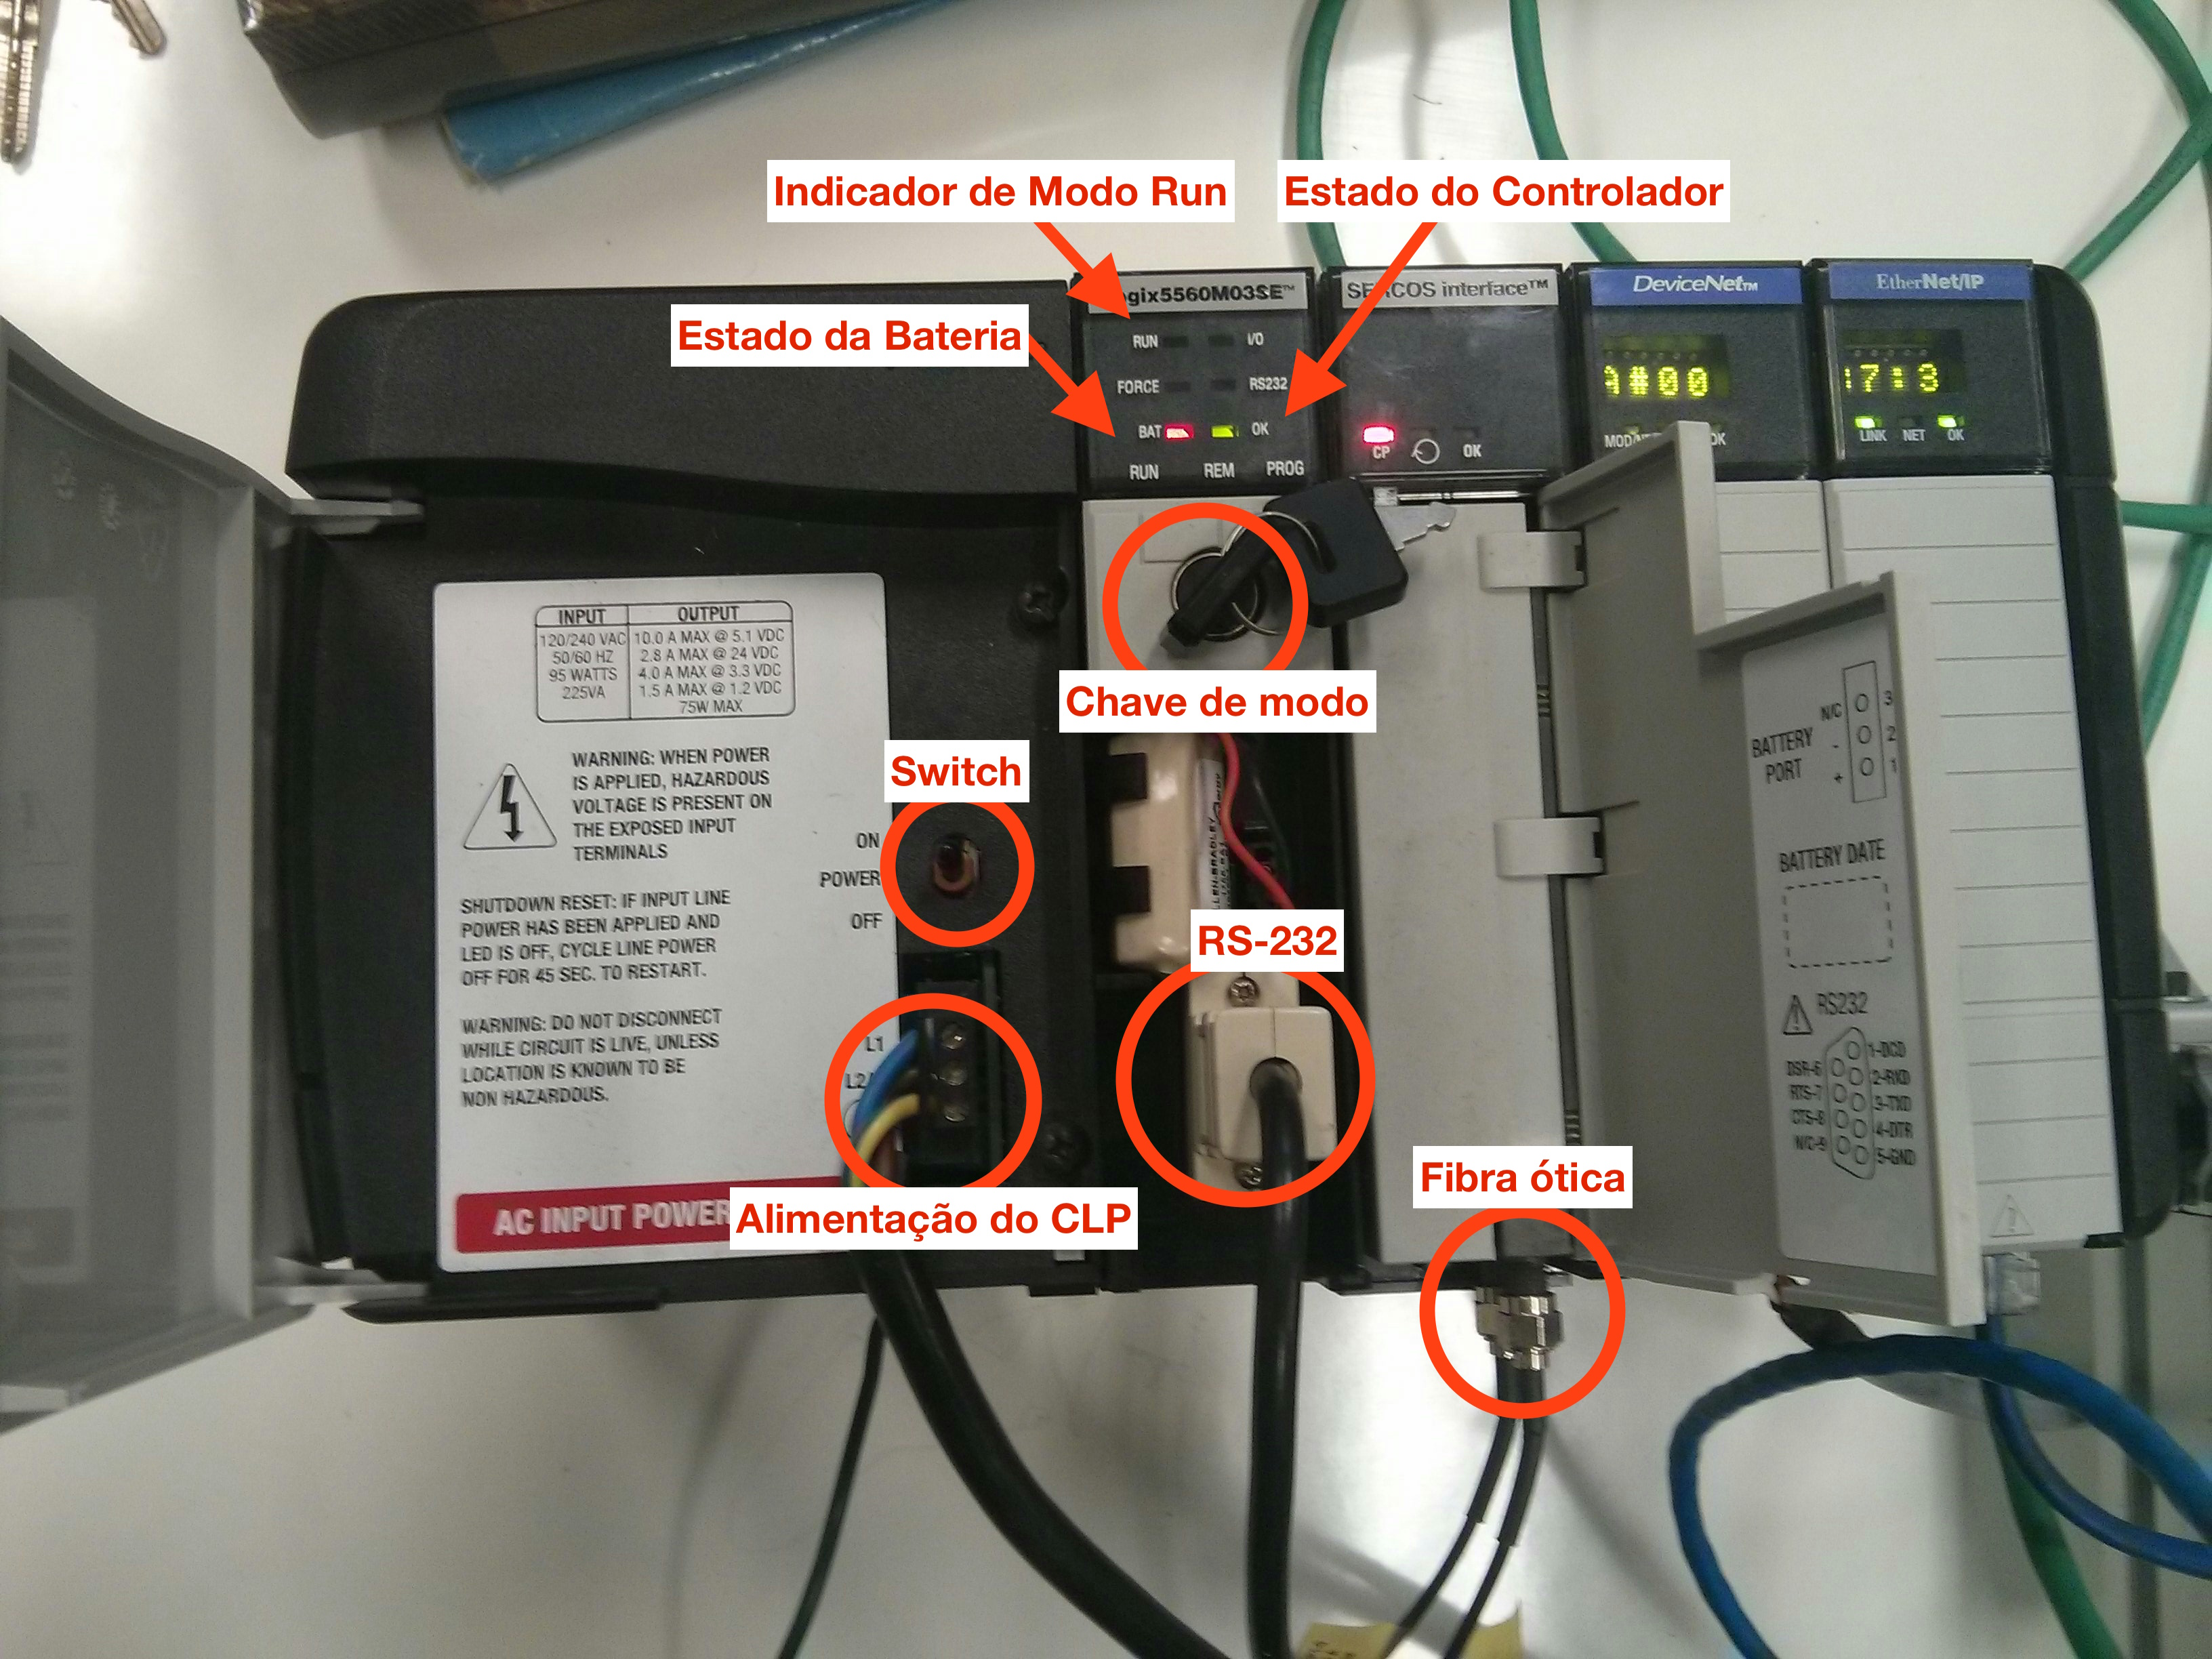
\includegraphics[width=0.9\textwidth]{figures/hardware/CLP.jpg}
    \caption{CLP com identificação de elementos\label{CLPcomentado}}
\end{figure}

\paragraph{} O controlador lógico-programável (CLP - ver Figura \ref{CLPcomentado}) é a espinha dorsal da bancada. Ele é responsável por executar os comandos de controle vindos do computador sobre todos os elementos que estão conectados a ele.
\paragraph{} O CLP utilizado é fabricado pela \textit{Allen Bradley}, modelo Logix5560M03SE. Tal modelo possui memória lógica e de dados de 750 KiB, e memória de \textit{I/O} de 494 KiB. Há quatro módulos no \textit{chassis} do controlador:
\begin{itemize}
  \item O próprio controlador;
  \item \textit{SERCOS Interface};
  \item DeviceNET;
  \item EtherNet/IP.
\end{itemize}
\paragraph{} Além dos módulos, o controlador ainda possui um \textit{switch} liga/desliga presente no \textit{chassis}. No módulo Logix, há uma chave responsável por alterar o modo de funcionamento do mesmo. As posições possíveis dessa chave são:
\begin{itemize}
  \item RUN;
  \item REM;
  \item PROG;
\end{itemize}
\paragraph{} Na prática, o modo REM se divide em dois modos: REM RUN e REM PROG. A maneira de se diferenciar os dois é observar, no módulo Logix, o estado do LED indicador de modo RUN quando a chave estiver na posição REM.
\paragraph{} No modo RUN, o controlador apenas roda o programa presente em sua memória; não há qualquer comunicação remota. No modo PROG, o controlador não roda nenhum programa; ele apenas pode receber um novo código. Nos modos REM, há a comunicação com o computador, permitindo verificar valores de variáveis de interesse e alterar, se necessário, o programa a ser rodado pelo controlador. O programa presente no controlador, em modo REM, só roda o código se estiver no modo REM RUN; se for necessário atualizar o programa, o modo deve ser o REM PROG.

\subsubsection{DeviceNET}
\paragraph{} O DeviceNET é a rede responsável por estabelecer a conexão do CLP com os sensores indutivos. A rede é alimentada com 24 Volts externa, pois o módulo DeviceNET não fornece tal alimentação.
\paragraph{} A rede DeviceNET também está conectada a um módulo de saídas, o \textit{CompactBlock I/O} (Figura \ref{CBcomentado} ). Esse bloco, na presente configuração, apenas transmite a alimentação da fonte de 24 V para os sensores e o módulo DeviceNET. A alimentação da rede também foi conectada à alimentação da câmera.

\begin{figure}[!ht]
  \centering
    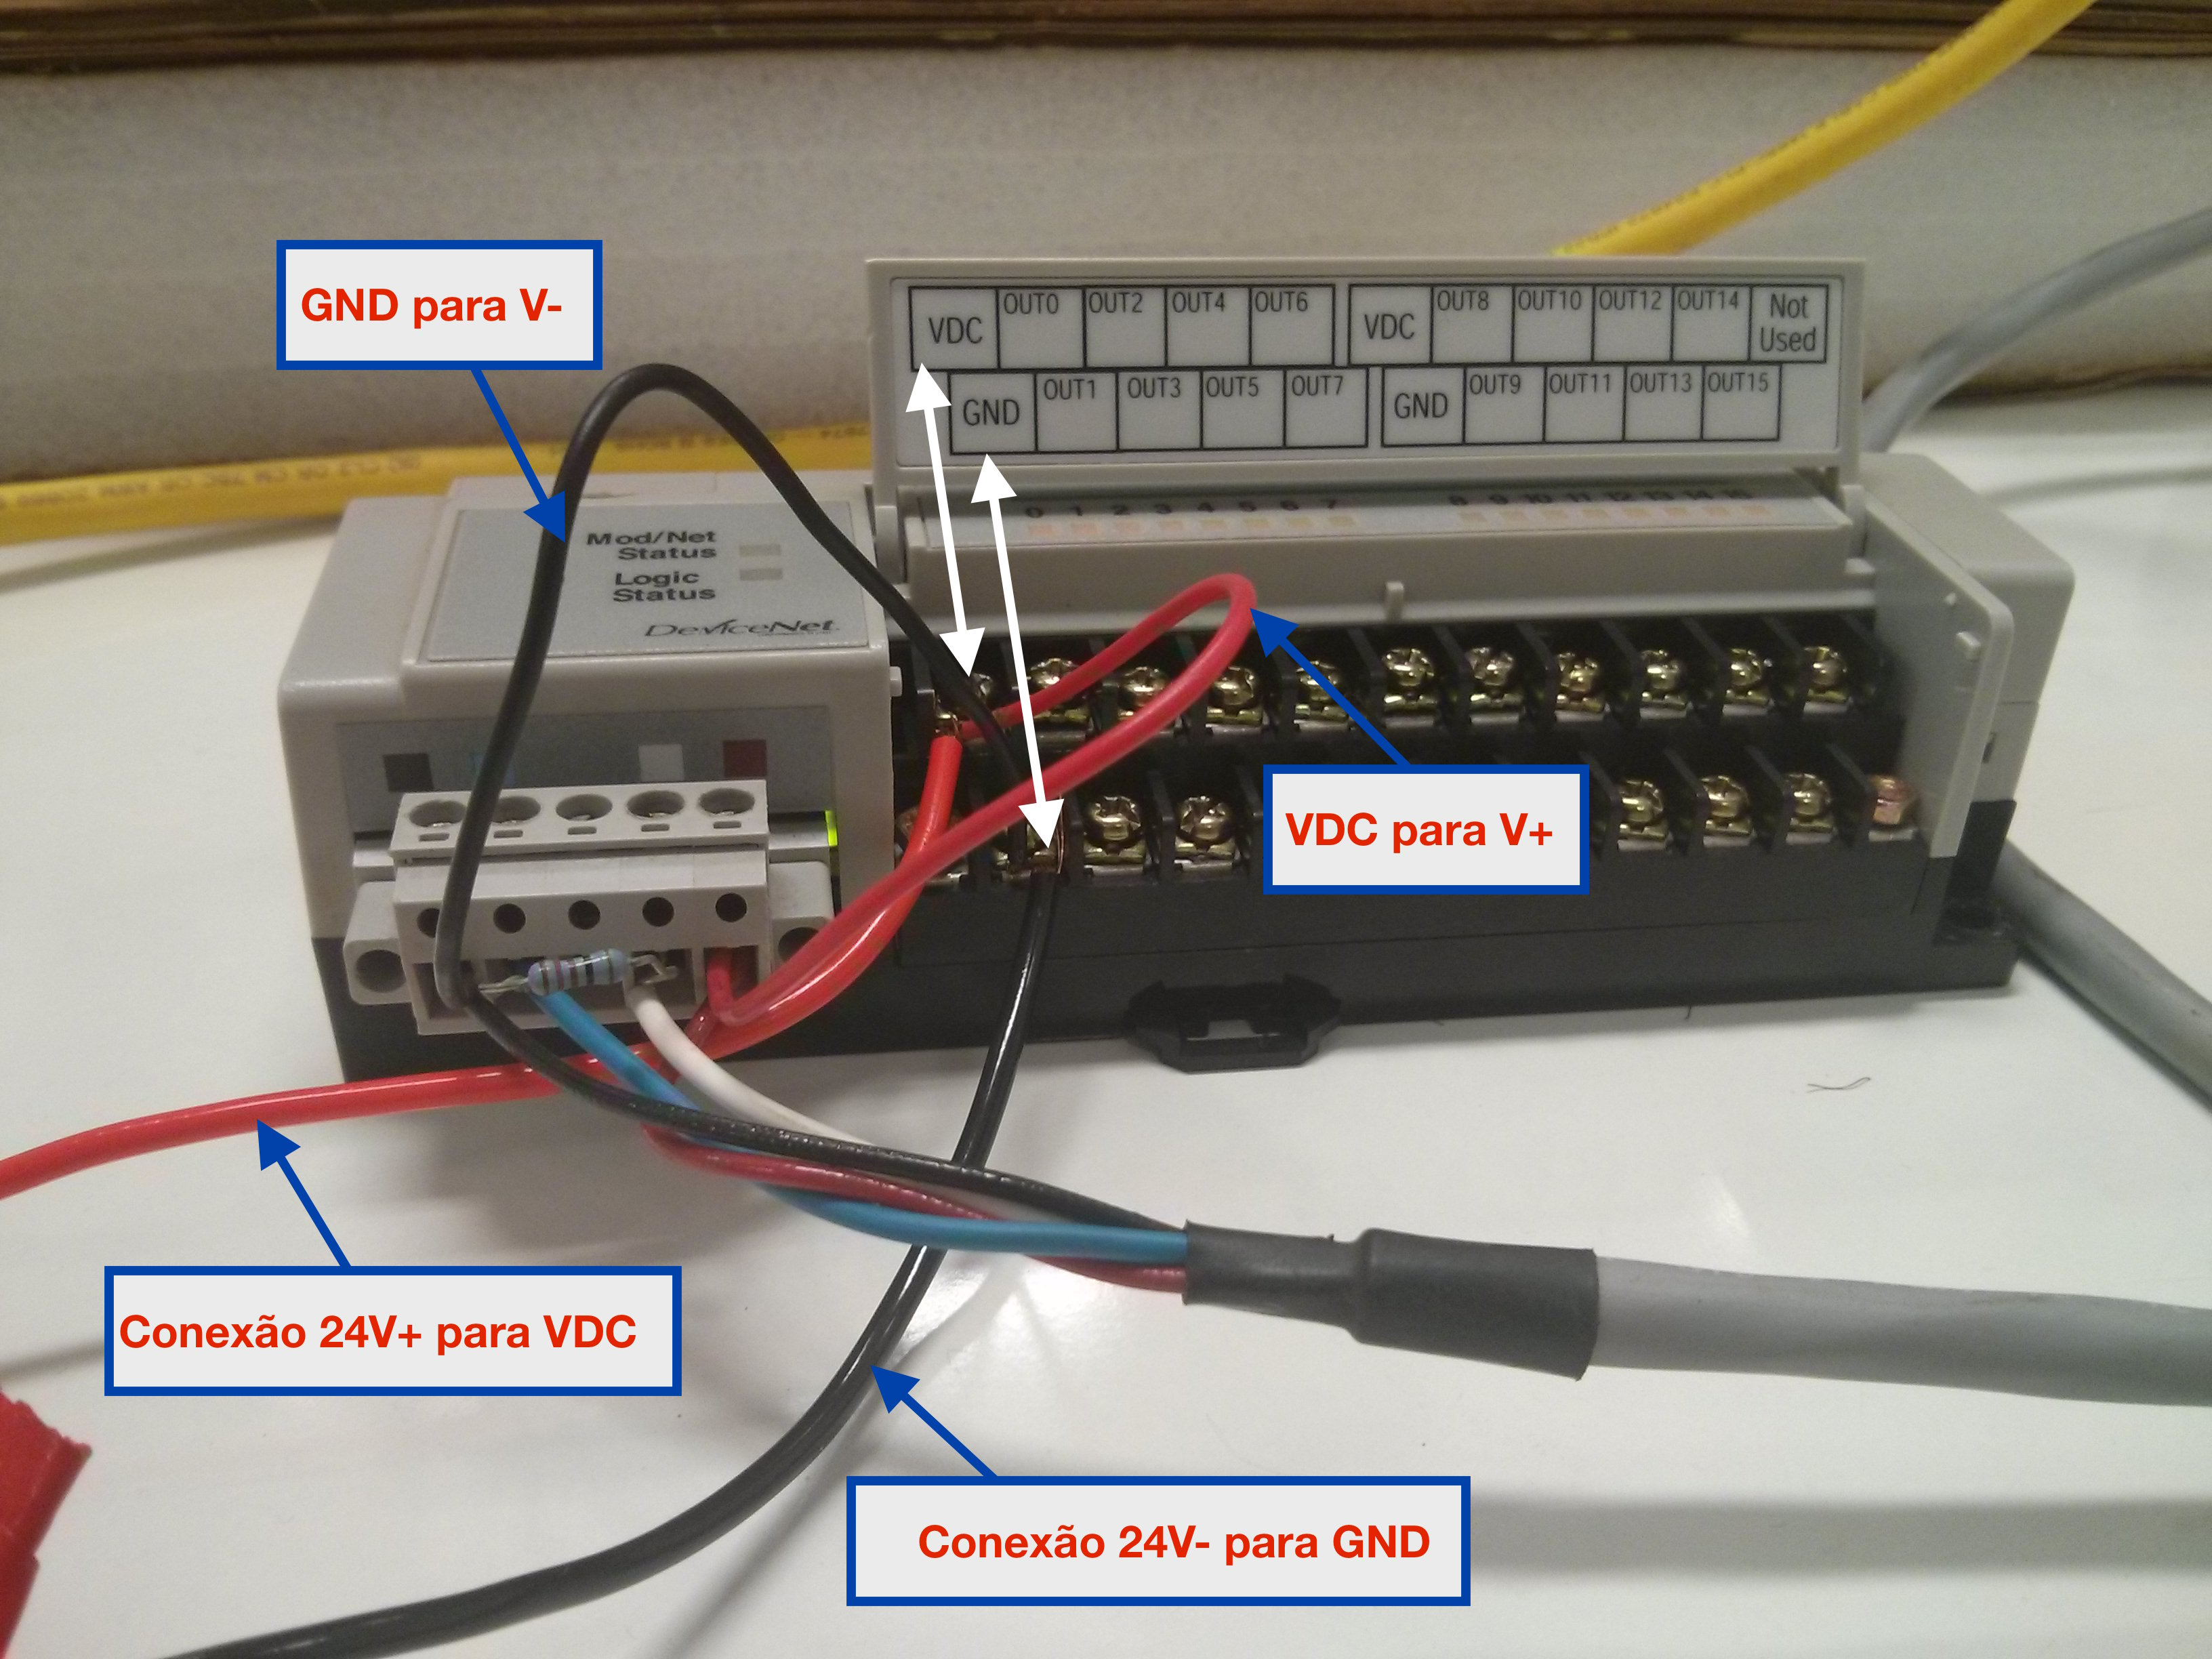
\includegraphics[width=0.9\textwidth]{figures/hardware/COMPACTBLOCK.jpg}
    \caption{CompactBlock com identificação de elementos\label{CBcomentado}}
\end{figure}

\subsubsection{Sensores Indutivos}
\paragraph{} Os sensores indutivos são elementos detectores de presença, particularmente de objetos metálicos. Eles funcionam através da variação de campo magnético ocasionada pela presença do objeto a ser identificado. Tal variação de campo magnético provoca uma variação de corrente dentro do sensor, alterando seu estado.
\paragraph{} Na presente bancada, há 6 sensores indutivos da família 871TM, fabricados pela \textit{Allen Bradley}. Eles são alimentados com tensão de 24 V, que está dentro dos limites padrão. São sensores feitos de aço, adaptados a ambientes industriais.

\subsubsection{Câmera}
\begin{table}[!ht]
  \centering
  \begin{tabular}{|c|c|}
    \hline Cor do Fio & Descrição \\ 
    \hline Amarelo & RS-232 TX \\ 
    \hline Cinza & Remote Teach \\ 
    \hline Laranja & Product Change \\
    \hline Rosa & External Trigger \\ 
    \hline Preto & Discrete I/O \#1 \\ 
    \hline Vermelho & Discrete I/O \#2 \\ 
    \hline Branco & Discrete I/O \#3 \\ 
    \hline Azul-Claro & Discrete I/O \#4 \\ 
    \hline Violeta & RS-232 RX \\ 
    \hline Verde & RS-232 Signal Ground \\ 
    \hline Azul & Common (Signal Ground) \\ 
    \hline Marrom & 10-30V DC \\ \hline  
  \end{tabular}
  \caption{Fiação da câmera\label{FioCamera}} 
\end{table}

\subsection{Cuidados com as conexões e com o controlador}
\paragraph{} Para que o sistema funcione corretamente, alguns cuidados devem ser tomados:
\begin{enumerate}
  \item A rede DeviceNET deve ser alimentada corretamente; caso contrário, o módulo DeviceNET emitirá uma mensagem de erro \textit{``No Network Power''}; caso essa mensagem seja mostrada, os sensores indutivos também não estarão alimentados, e não funcionarão.
  \item O \textit{switch} liga/desliga do controlador é protegido por uma tampa. É recomendável que, com o controlador em operação, que esta tampa esteja fechada.
  \item Atentar para o estado do disjuntor industrial; ele deve estar ligado para que o motor funcione.
  \item Não retirar a chave de modo do controlador; sem ela, pode ser impossível carregar um novo programa para o controlador ou mesmo rodar um programa já carregado.
\end{enumerate}

\section{Criando um novo programa no RSLogix}
\paragraph{} Esta seção tem por objetivo demonstrar os passos para criar um programa novo e fazer as configurações básicas para que um programa simples possa ser executado. Aqui, já se considera que o RSLinx tenha sido utilizado para verificar as conexões dos dispositivos. Note que, quando não mencionado o nome para se dar a um programa ou dispositivo, é livre a escolha, contanto que seja consistente.
\subsection{Adicionando dispositivos}
\begin{enumerate}
	\item \textbf{Crie um novo controlador (Ctrl+N) e configure da seguinte maneira}
	\begin{figure}[!ht]
  \centering
    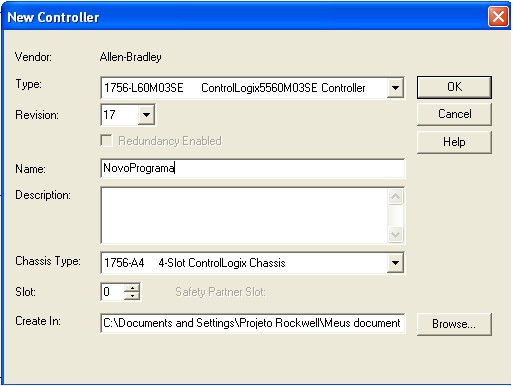
\includegraphics[width=0.6\textwidth]{figures/software/step01}
\end{figure}
	\item \textbf{Adicione o driver 2094-AC05-MP5 no SERCOS} 

\begin{minipage}[!ht]{\linewidth}
      \centering
      \begin{minipage}{0.45\linewidth}
          \begin{figure}[H]
              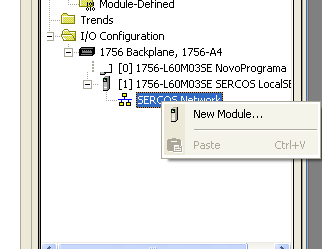
\includegraphics[width=\linewidth]{figures/software/step02}
          \end{figure}
      \end{minipage}
      \hspace{0.05\linewidth}
      \begin{minipage}{0.45\linewidth}
          \begin{figure}[H]
              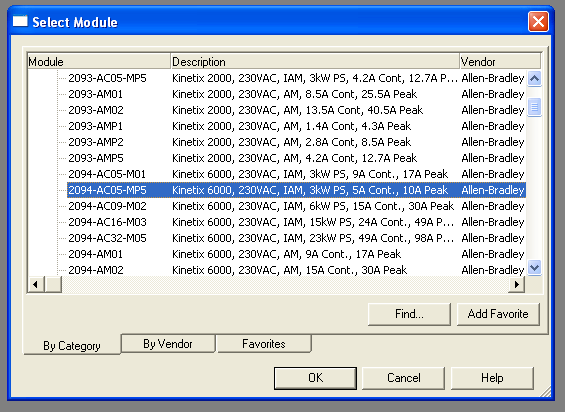
\includegraphics[width=\linewidth]{figures/software/step03}
          \end{figure}
      \end{minipage}
      \begin{minipage}{0.45\linewidth}
          \begin{figure}[H]
              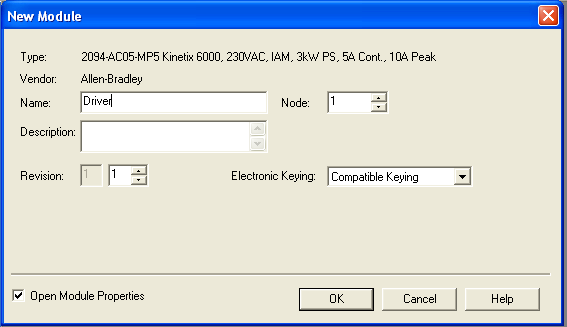
\includegraphics[width=\linewidth]{figures/software/step04}
          \end{figure}
      \end{minipage}
  \end{minipage}
  \item \textbf{Abra as propriedades do módulo 2094-AC05-MP5: } Agora, vá na aba \textit{Associated Axes} e clique em \textit{New Axis}. Dê um nome ao eixo e confirme. Após isso, associe o eixo ao nó 1. Veja figuras abaixo para clarificar dúvidas. 
  
 	\begin{minipage}[!ht]{\linewidth}
      \centering
      \begin{minipage}{0.45\linewidth}
          \begin{figure}[H]
              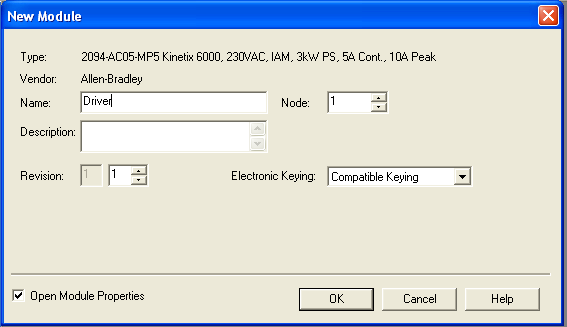
\includegraphics[width=\linewidth]{figures/software/step04}
          \end{figure}
      \end{minipage}
      \hspace{0.05\linewidth}
      \begin{minipage}{0.45\linewidth}
          \begin{figure}[H]
              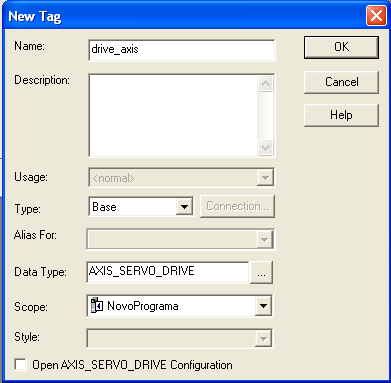
\includegraphics[width=\linewidth]{figures/software/step05}
          \end{figure}
      \end{minipage}
      \begin{minipage}{0.45\linewidth}
          \begin{figure}[H]
              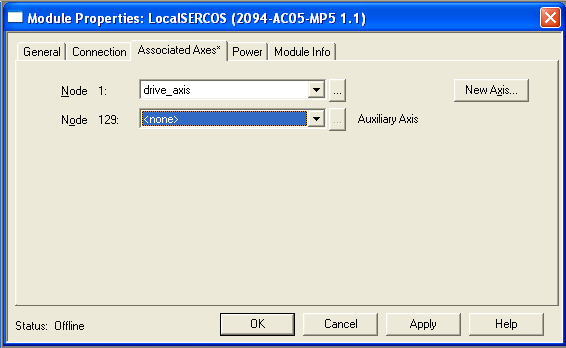
\includegraphics[width=\linewidth]{figures/software/step06}
          \end{figure}
      \end{minipage}

  \end{minipage}

  \item \textbf{Crie um motion group: } Vá em \textit{Motion Group} e clique em \textit{New Motion Group}. Dê um nome e clique e OK.


   	\begin{minipage}[!ht]{\linewidth}
      \centering
      \begin{minipage}{0.45\linewidth}
          \begin{figure}[H]
              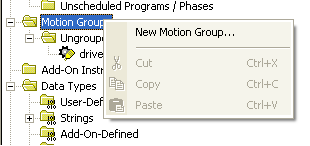
\includegraphics[width=\linewidth]{figures/software/step11}
          \end{figure}
      \end{minipage}
      \hspace{0.05\linewidth}
      \begin{minipage}{0.45\linewidth}
          \begin{figure}[H]
              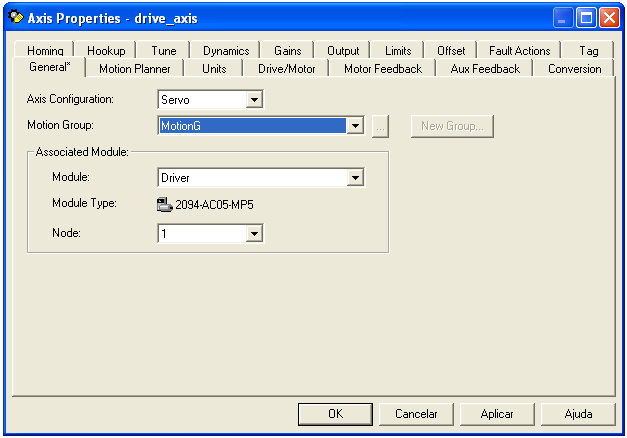
\includegraphics[width=\linewidth]{figures/software/step12}
          \end{figure}
      \end{minipage}
  \end{minipage}
  
  \item \textbf{Associar eixo ao Motion Group: } nas propriedades do eixo criado, adicione ao grupo. O resultado deve mostrar o eixo dentro do grupo de movimento.
  
  \begin{figure}[H]
  	\centering
  	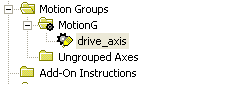
\includegraphics[width=0.3\linewidth]{figures/software/step13}
  \end{figure}
  
  \item \textbf{Associar motor ao driver: } Vá nas propriedades do eixo, seleciona a aba \textit{Drive/Motor}, clique em \textit{Change Catalog}, selecione MPL-A310F-S e clique em OK.
  
  \begin{figure}[H]
  \centering
              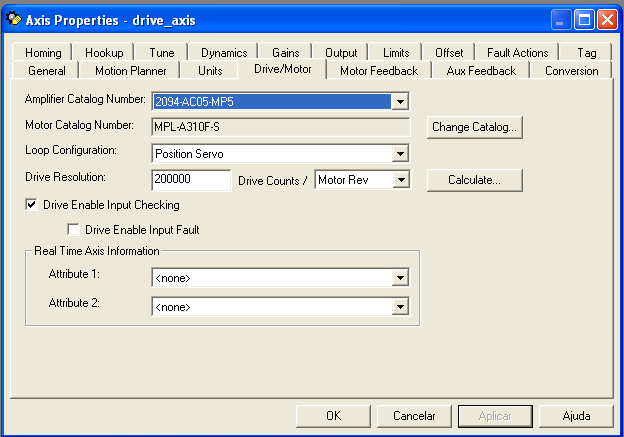
\includegraphics[width=0.5\linewidth]{figures/software/stepXY}
          \end{figure}
  \item \textbf{Adicionar DeviceNet: } No backplane, clique em novo módulo. Daí, vá em \textit{Communications} e adicione o 1756-DNB. Escolha a revisão 7 e clique em OK. Na sub-revisão, escolha 3 e pode clicar em OK para fechar as propriedades do módulo.
  
  \begin{minipage}[!ht]{\linewidth}
      \centering
      \begin{minipage}{0.45\linewidth}
          \begin{figure}[H]
              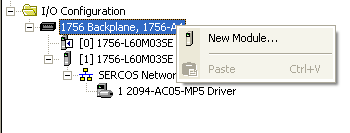
\includegraphics[width=\linewidth]{figures/software/step07}
          \end{figure}
      \end{minipage}
      \hspace{0.05\linewidth}
      \begin{minipage}{0.45\linewidth}
          \begin{figure}[H]
              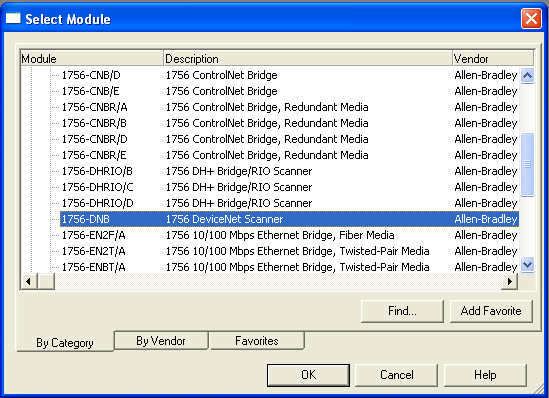
\includegraphics[width=\linewidth]{figures/software/step08}
          \end{figure}
      \end{minipage}
      \begin{minipage}{0.45\linewidth}
          \begin{figure}[H]
              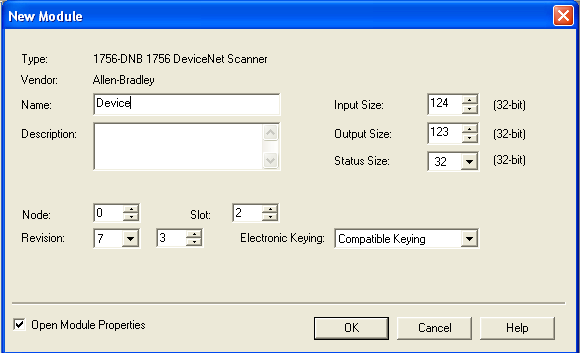
\includegraphics[width=\linewidth]{figures/software/step09}
          \end{figure}
      \end{minipage}
  \end{minipage}
  
  \item \textbf{Adicionar módulo Ethernet/IP: } crie um novo módulo no backplane e então vá em \textit{Communications} e selecione 1756-ENBT/A e use revisão 4 com sub-revisão 1. O endereço IP pode ser definido como 192.168.0.4, por exemplo. (ou não? é definido no RSLinx?)
  
       \begin{figure}[H]
       \centering
              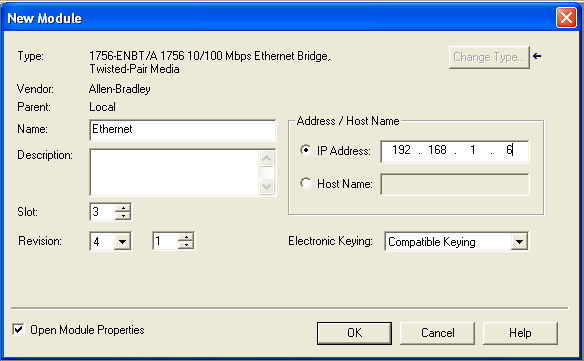
\includegraphics[width=0.5\linewidth]{figures/software/step10}
          \end{figure}
\end{enumerate}

\paragraph{} A configuração dos dispositivos foi terminada (talvez o que falte seja a câmera... não sei se é necessário que ela seja adicionada no programa).

\subsection{Programando}
\begin{enumerate}
	\item \textbf{Abra o programa principal: } deve-se observar uma linha em branco de ladder.
	\begin{figure}[H]
       \centering
              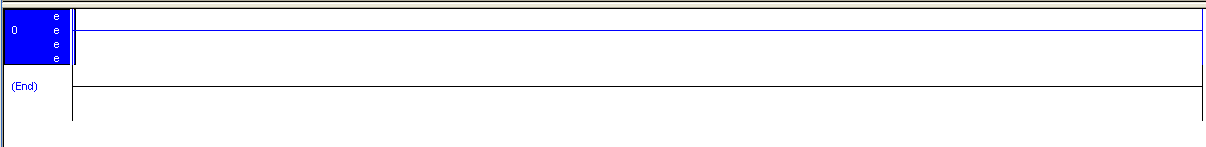
\includegraphics[width=0.8\linewidth]{figures/software/step14}
          \end{figure}
     \item \textbf{Crie o programa principal: } a Figura \ref{mainRoutine} mostra o programa principal. Note que as variáveis \texttt{MAJ\_1} e \texttt{MAJ\_2} devem ser criadas. Pode-se fazer isso clicando em cada uma delas com o botão esquerdo e escolhendo a opção apropriada. Configurações completas para o bloco MAJ estão na Figura \ref{majConf}. O bloco MSO liga o servomotor e MAJ muda a velocidade, veja a documentação dos blocos para maiores informações. O programa principal faz o carrinho se mexer em um sentido quando o sensor 2 for ativado e em outro sentido quando o sensor 5 for ativado.
     \begin{figure}[H]
       \centering
              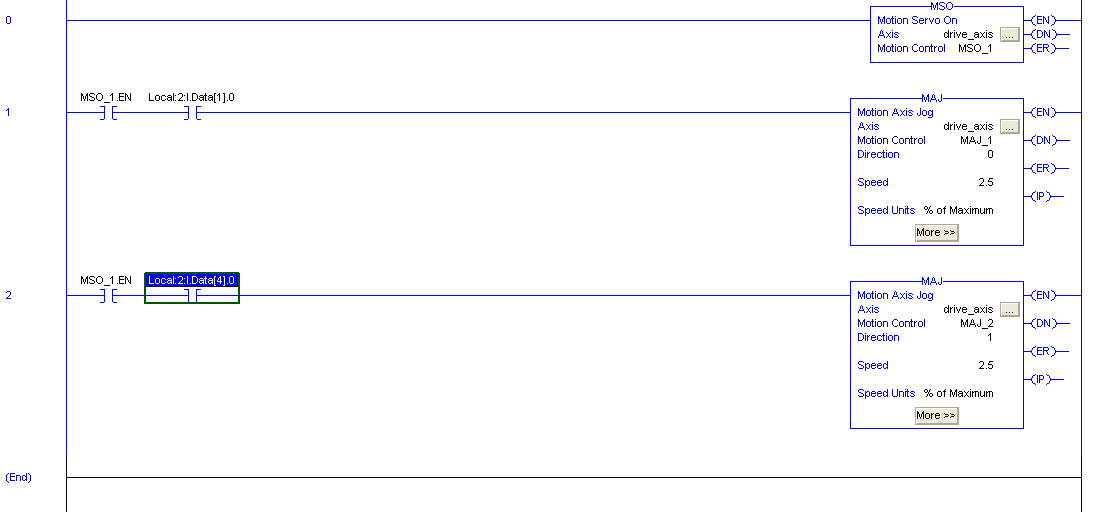
\includegraphics[width=0.9\linewidth]{figures/software/step16}
              \caption{Programa principal\label{mainRoutine}}
          \end{figure}
        \begin{figure}[H]
       \centering
              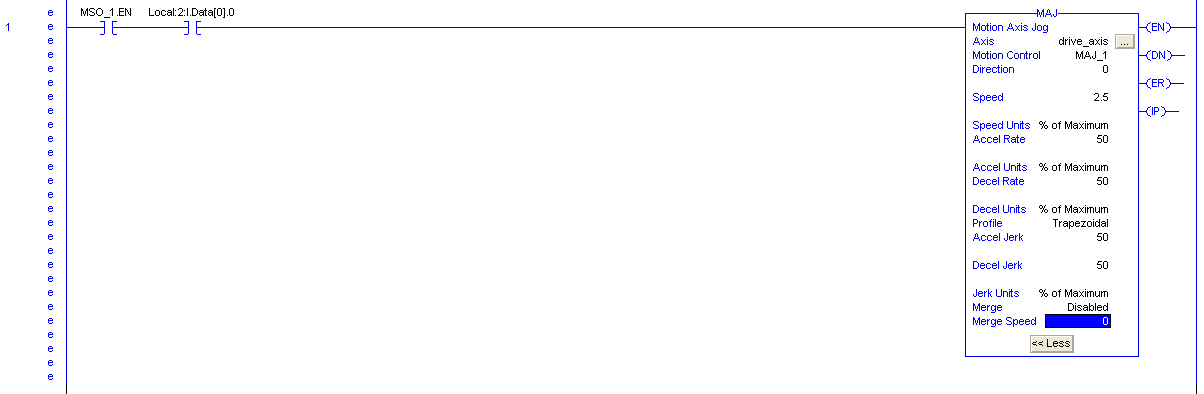
\includegraphics[width=0.9\linewidth]{figures/software/step15}
              \caption{Configurações do MAJ\label{majConf}}
          \end{figure}
     \item \textbf{Crie o programa que liga a rede DeviceNet: } crie um novo programa dentro de \textit{MainTask} e após isso crie uma rotina do tipo Ladder Diagram dentro desse novo programa. O programa que deve ser criado está na Figura \ref{deviceRoutine}.
     
       \begin{minipage}[!ht]{\linewidth}
      \centering
      \begin{minipage}{0.45\linewidth}
          \begin{figure}[H]
              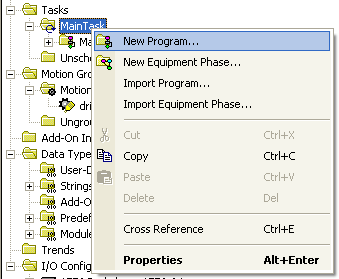
\includegraphics[width=\linewidth]{figures/software/step17}
          \end{figure}
      \end{minipage}
      \hspace{0.05\linewidth}
      \begin{minipage}{0.45\linewidth}
          \begin{figure}[H]
              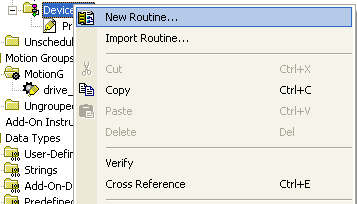
\includegraphics[width=\linewidth]{figures/software/step18}
          \end{figure}
      \end{minipage}
  \end{minipage}
  
       \begin{figure}[H]
       \centering
              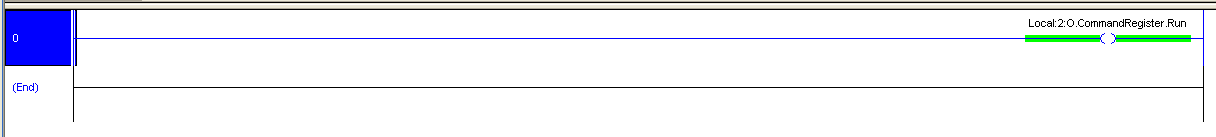
\includegraphics[width=0.9\linewidth]{figures/software/step19}
              \caption{Programa que liga DeviceNet\label{deviceRoutine}}
          \end{figure}
          
     \item \textbf{Torne a rotina criada uma rotina principal: } vá nas propriedades do programa, selecione a aba \textit{Configuration} e escolha o nome da sua rotina criada como a rotina \textit{Main}.
     
     \begin{figure}[H]
       \centering
              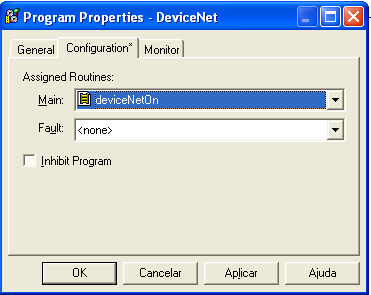
\includegraphics[width=0.5\linewidth]{figures/software/step20}
          \end{figure}
     
     \item \textbf{Crie uma rotina de segurança: } crie um novo programa, crie uma nova rotina do tipo Ladder Diagram e então marque essa rotina como principal. Após isso, programe conforme a Figura \ref{seguranca}. Nessa rotina, o motor para caso certos sensores sejam ativados.
     
     \begin{figure}[H]
       \centering
              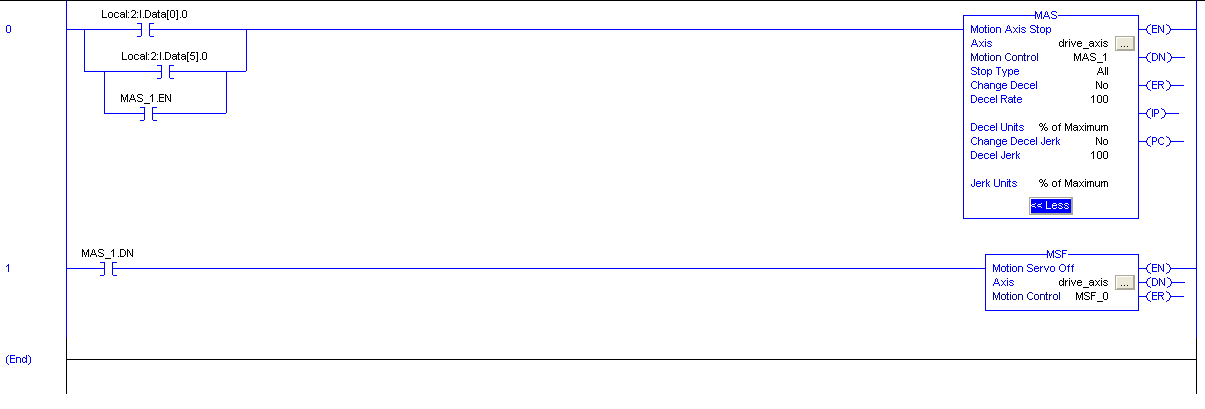
\includegraphics[width=0.9\linewidth]{figures/software/step21}
              \caption{Rotina de segurança\label{seguranca}}
          \end{figure}
     
     \item \textbf{Execute o programa: } Para rodar o programa pela primeira vez, clique no menu ``Communications'' e depois ``Who Active''. Para usar o RS para comunicação, selecione AB\_DF1-1, DF1 e depois clique em download. Na primeira vez, lembre-se de verificar a opção ``Designate this controller as CST master''.
	
	\begin{figure}[H]
       \centering
              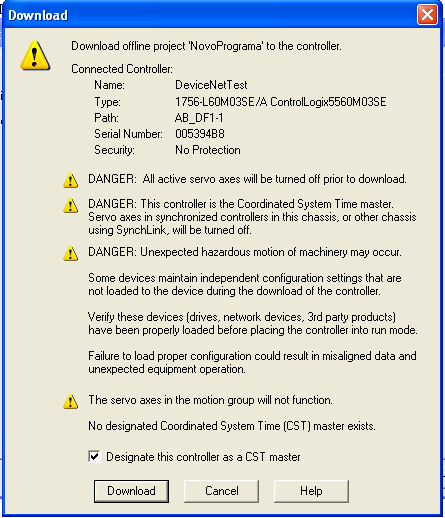
\includegraphics[width=0.9\linewidth]{figures/software/step23}
              \caption{Mensagem que aparece quando se executa o programa e opção que aparece pela primeira vez\label{mensagemRodar}}
          \end{figure}
\end{enumerate}

\subsection{Programando II: Texto Estruturado}
\paragraph{} O controlador presentemente utilizado permite que programas razoavelmente grandes escritos em \textit{ladder} possam ser executados e guardados em sua memória. O controlador 1560 possui cerca de 760 kB de memória. Porém, pode ser necessário se utilizar uma linguagem mais simples, uma vez que o espaço pode ser um problema e a linguagem \textit{ladder} não é conveniente em casos que muitos parâmetros devem ser alterados por fora, ao mesmo tempo. Neste caso, torna-se interessante o uso de uma outra linguagem, puramente textual. Essa linguagem é conhecida como texto estruturado (\textit{Structured Text}).
\paragraph{} Para se utilizar o texto estruturado, basta seguir os seguintes passos:
%% TODO pegar figuras
\begin{enumerate}
  \item \textbf{Criar uma nova rotina: } Esse passo é semelhante à criação de uma nova rotina em \textit{ladder}, mas a linguagem a ser selecionada é o texto estruturado.
  
  \item \textbf{Programação em texto: } Para se programar em texto estruturado, deve-se ter em mente que o raciocínio é o mesmo empregado para o \textit{ladder}; as \textit{tags} utilizadas devem existir, por exemplo. Caso seja escrita uma \textit{tag} ainda inexistente, o \textit{RSLogix 5000} irá sublinhar a \textit{tag} com uma linha vermelha, sinalizando que há um erro; basta clicar com o botão direito do \textit{mouse} no texto e adicionar a \textit{tag}, clicando na opção \textit{``New Tag...''}. A partir desse passo, as configurações da nova \textit{tag} são feitas do mesmo modo que na programação \textit{ladder}.
  
  \item \textbf{Texto estruturado x \textit{ladder}: } Embora a maioria das instruções \textit{ladder} possua um equivalente normal em texto estruturado, há algumas instruções que devem ser notadas por não existir em texto estruturado, por exemplo; há outras instruções que existem em texto, mas não em \textit{ladder}. A tabela \ref{ladderstrel} mostra alguns exemplos:
  \begin{table}[!ht]
    \centering
    \caption{Relações entre instruções \textit{ladder} e texto estruturado \label{ladderstrel}}
    \begin {tabular}{|c|c|}
    \hline
      Instrução \textit{ladder} & Instrução em texto \\ \hline
      -( )- [OTE] & A [:=] X \\ \hline
      -(L)- [OTL] & A := 1 \\ \hline
      -(U)- [OTU] & A := 0 \\ \hline
      %% TODO achar uma formatação melhor
      -[ ]- [XIC] & \shortstack{IF A = 1 THEN\\;Code\\END\_IF;} \\ \hline
      -[/]- [XIO] & \shortstack{IF A = 0 THEN\\;Code\\END\_IF;} \\ \hline
      Timer On Delay (TON) & TONR(TIME_TAG) \\ \hline
      
    \end{tabular}
  \end{table}
\end{enumerate}

\section{Câmera}
\subsection{Configurando a câmera}
\paragraph{} Para que a câmera possa ser utilizada, é necessário que se estabeleça uma comunicação entre ela, o computador e o controlador, para que seja possível efetuar sua calibração e seu uso como sensor visual presente no experimento. Tendo em vista este objetivo, faz-se necessária a configuração de uma rede, que, neste experimento, será uma rede \textit{Ethernet} com um \textit{switch}. Os passos a seguir descrevem essa configuração.
\begin {enumerate}
  \item \textbf{Configuração física da rede: } A câmera, o controlador e o computador devem estar ligados entre si através de cabos \textit{Ethernet}. Todos os cabos dever ser conectados ao \textit{switch}.
  \item 
  \item
  \item 
\end{enumerate}

\subsection{Calibração}
\paragraph{} A câmera permite fazer medidas de distâncias em pixels. De forma a se converter essa distância para milímetros, uma barra de alumínio com marcas e tamanho conhecido é utilizada. É importante primeiro calibrar o sistema, para se saber se há deformação de pixels significante ao longo da distância de interesse. No PresencePlus P4 GEO 1.3, um programa com imagem de referência é feito, conforme Figura .... A barra de alumínio atualmente utilizada tem comprimento total de $532$mm. Algumas marcas foram feitas e a Tabela \ref{relacoesmmpx} apresenta os resultados para cada seção. A distância entre duas marcas é de 10cm.

\begin{table}[!ht]
\centering
\caption{Relações mm/px para diferentes seções da barra de alumínio \label{relacoesmmpx}}
	\begin{tabular}{|c|c|c|c|}
	\hline
		Seção 1 & Seção 2 & Distância (px) & mm/px\\ \hline
		P0 & P10 & 160 & 0.625\\ \hline
		P10 & P20 & 173 & 0.578\\ \hline
		P20 & P30 & 176 & 0.568\\ \hline
		P30 & P40 & 173 & 0.578\\ \hline
		P40 & P50 & 163 & 0.613\\ \hline
		P0 & PEND & 893 & 0.596\\ \hline
	\end{tabular}
\end{table}

\paragraph{} O maior desvio da quantidade de milímetros por pixels das seções em relação à da barra inteira é de aproximadamente 4.93\%. Há algumas imprecisões na maneira como os traços foram desenhados e é possível que o erro seja menor.

\end{document}
